\documentclass[14pt]{extarticle}
\usepackage[margin=1in]{geometry}
\usepackage{graphicx}
\usepackage{booktabs}
\usepackage{amsmath}
\usepackage{amssymb}
\usepackage{float}
\usepackage{caption}
\usepackage{setspace}
\usepackage[most]{tcolorbox}
\usepackage{hyperref}
\captionsetup{font=small, labelfont=bf, skip=4pt}
\setstretch{1.15}
\hypersetup{
  colorlinks=true,
  linkcolor=black,
  citecolor=blue,
  urlcolor=blue
}
\graphicspath{{../figures/}}

\newtcolorbox{explain}{%
  colback=black!3,
  colframe=black!25,
  boxrule=0.5pt,
  arc=1pt,
  left=8pt,
  right=8pt,
  top=4pt,
  bottom=4pt,
  before skip=6pt,
  after skip=8pt,
  fontupper=\normalsize
}

\title{Debiasing Facial Detection\\[0.2em]
\large by Learned Latent Structure}
\author{}
\date{30 September 2026}

\begin{document}
\maketitle

\begin{abstract}
\noindent
A face detector trained on a biased set of photographs can be nearly perfect on the mixture it was shown and still assign much lower face probability to faces that mixture rarely contains. We train that detector twice. First, faces and non-faces are drawn uniformly into a standard CNN. Second, the same convolutional trunk becomes the encoder of a variational autoencoder: it still says whether an image is a face and, for faces, also explains the image through a hundred-dimensional Gaussian code. Once an epoch, faces that land in sparse regions of that code are drawn more often. On the four-group test set, mean predicted face probability becomes more even across light and dark groups under the debiased model. Method: debiasing variational autoencoder of Amini et al.~\cite{amini2019}.
\end{abstract}

\clearpage
\tableofcontents
\clearpage

\section{Bias, without a label for it}
\subsection{Latent variables}
Given an image, a detector returns the probability that it is a face. Skin tone, gender, pose, and hats are not labels in that task. They are latent variables: they shape the image, and training does not record them. A classifier is biased if its decision changes once such a latent feature is revealed. High average accuracy can hide that, because averages are taken on the training distribution.

\subsection{Hand annotation}
Most faces in CelebA~\cite{liu2015}, the positive training set, are light-skinned women. A network trained by uniform draws spends most of its steps on that appearance. One repair is to annotate subclasses and even them out by hand. That requires labeling a great deal of data, and knowing in advance which biases to look for. Pose, occlusion, hats, and glasses are missed unless someone annotated them. An alternative, followed below, is to learn those features without annotation and then train the classifier with respect to what was learned.

\section{What the two sets look like}
\subsection{Training images}
Positive training images are CelebA faces~\cite{liu2015}. Negative training images are non-human ImageNet categories~\cite{deng2009}. Both are \(64\times 64\) RGB. Training uses batch size \(32\). No demographic column is read during training.

\begin{figure}[H]
\centering
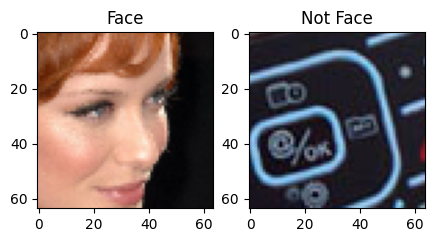
\includegraphics[width=0.72\textwidth]{train_face_not_face.png}
\caption{One positive and one negative training image, at the resolution the networks see.}
\end{figure}

\subsection{Test set}
Test images follow the Pilot Parliaments Benchmark style of Buolamwini and Gebru~\cite{buolamwini2018}: faces grouped by the Fitzpatrick scale and by sex into light female, light male, dark female, and dark male. Every test image is a face. Evaluation below reports each model's mean predicted face probability on each group.

\begin{figure}[H]
\centering
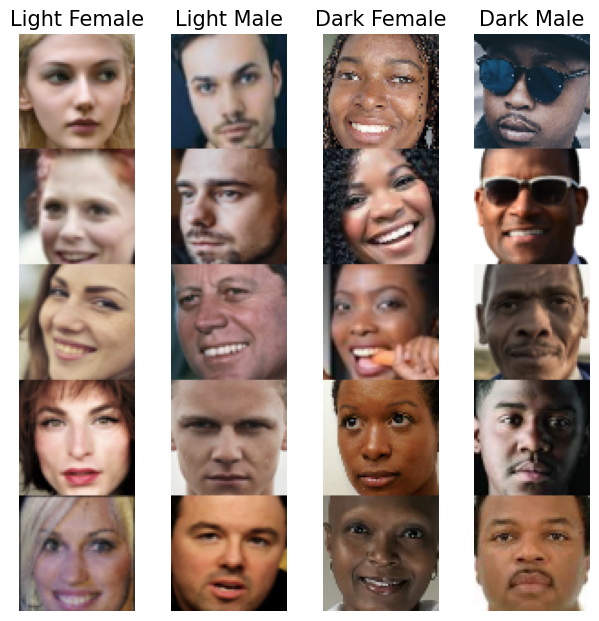
\includegraphics[width=0.88\textwidth]{test_set.png}
\caption{Test faces by demographic group. These four labels are not used in training.}
\end{figure}

\section{Standard CNN}
\subsection{Architecture}
Baseline is a convolutional neural network (CNN) with no latent code and no resampling. Each block is a convolution, a ReLU, and batch normalization. Spatial size halves at every block.

\begin{table}[H]
\centering
\begin{tabular}{llc}
\toprule
Block & Kernel & Output \\
\midrule
1 & \(5\times 5\), stride 2 & \(32\times 32\), 12 ch. \\
2 & \(5\times 5\), stride 2 & \(16\times 16\), 24 ch. \\
3 & \(3\times 3\), stride 2 & \(8\times 8\), 48 ch. \\
4 & \(3\times 3\), stride 2 & \(4\times 4\), 72 ch. \\
5 & linear, ReLU & 512 \\
6 & linear & 1 logit \\
\bottomrule
\end{tabular}
\caption{Standard CNN. Flattened map has \(4\cdot 4\cdot 72 = 1{,}152\) units.}
\end{table}

\subsection{Training}
Optimizer is Adam at \(5\times 10^{-4}\), batch size \(32\), two epochs, binary cross-entropy on the logit, and uniform minibatches.

\begin{figure}[H]
\centering
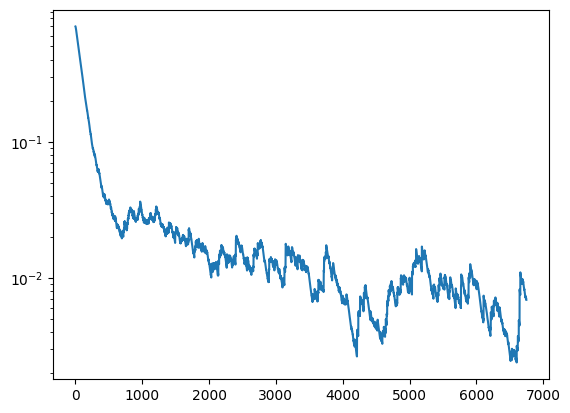
\includegraphics[width=0.62\textwidth]{cnn_training_loss.png}
\caption{CNN training loss, logarithmic vertical scale, both epochs.}
\end{figure}

On \(5{,}000\) fresh training images the CNN is right \(99.64\%\) of the time. On the demographic test set it assigns clearly higher mean face probability to light-skinned groups than to dark-skinned groups (Figure~\ref{fig:compare}). Training accuracy and that test gap sit side by side: the CNN was fit on CelebA, and CelebA does not look like the test set.

\section{Variational autoencoder}
Rarity has to be measured in some coordinate system. A variational autoencoder (VAE) learns one, with no labels on the factors.

\begin{figure}[H]
\centering
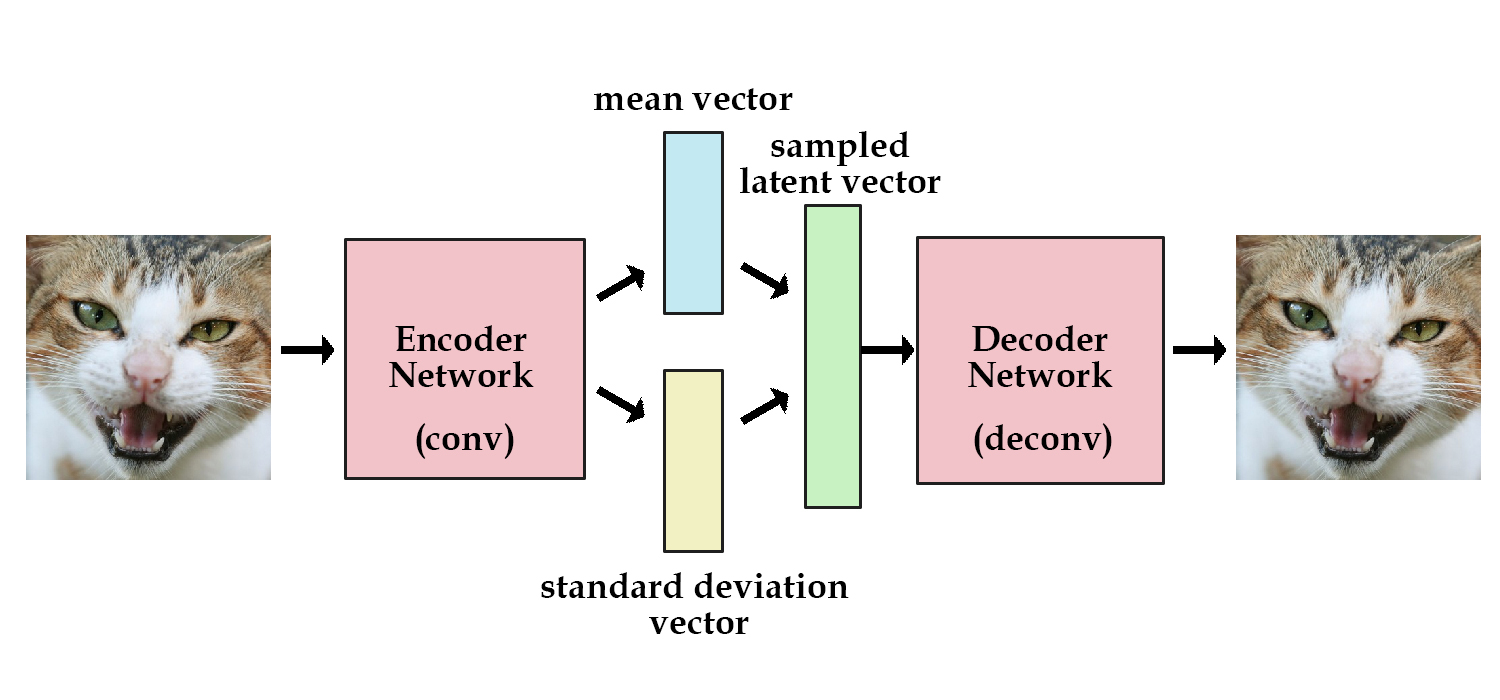
\includegraphics[width=\textwidth]{vae_schematic.jpg}
\caption{Encoder, mean, standard deviation, sampled code, decoder. Image is \(64\times 64\); each vector has length \(100\).}
\end{figure}

\subsection{Loss}
Encoder reads \(x\) and emits a mean \(\mu\) and a per-coordinate spread. A code \(z\) is drawn from that Gaussian and the decoder paints \(\hat x\). Both pieces enter the loss, because both are learned. Latent term measures how close \((\mu,\sigma)\) stays to a unit Gaussian, by the KL divergence
\[
L_{\mathrm{KL}}(\mu,\sigma)
=
\frac12\sum_{j=0}^{k-1}
\bigl(\sigma_j + \mu_j^2 - 1 - \log\sigma_j\bigr).
\]
Reconstruction term is pixelwise absolute deviation
\[
L_x(x,\hat x) = \lVert x-\hat x\rVert_1,
\]
averaged over channels, height, and width. With weight \(c = 5\times 10^{-4}\) on the latent term,
\[
L_{\mathrm{VAE}} = c\,L_{\mathrm{KL}} + L_x(x,\hat x).
\]
Coefficient \(c\) is a regularizer: it sets how hard the code is pulled toward the unit Gaussian.

\subsection{Reparameterization}
Sampling \(z\) inside the network has to leave a path for the gradient. Reparameterization draws noise that does not depend on the encoder, then shifts and scales it,
\[
\varepsilon\sim\mathcal{N}(0,I),
\qquad
z = \mu + \exp\bigl(\tfrac12\log\sigma\bigr)\circ\varepsilon.
\]
Sample is random, and the map from \((\mu,\log\sigma)\) to \(z\) is differentiable, so the whole network trains by backpropagation.

\section{Debiasing model (DB-VAE)}
A plain autoencoder does not classify. Classification needs a class output sharing the encoder trunk, so features used to recognize a face are features whose distribution gets rebalanced. That joint model is the DB-VAE: CNN trunk as encoder, plus decoder and resampling.

\begin{figure}[H]
\centering
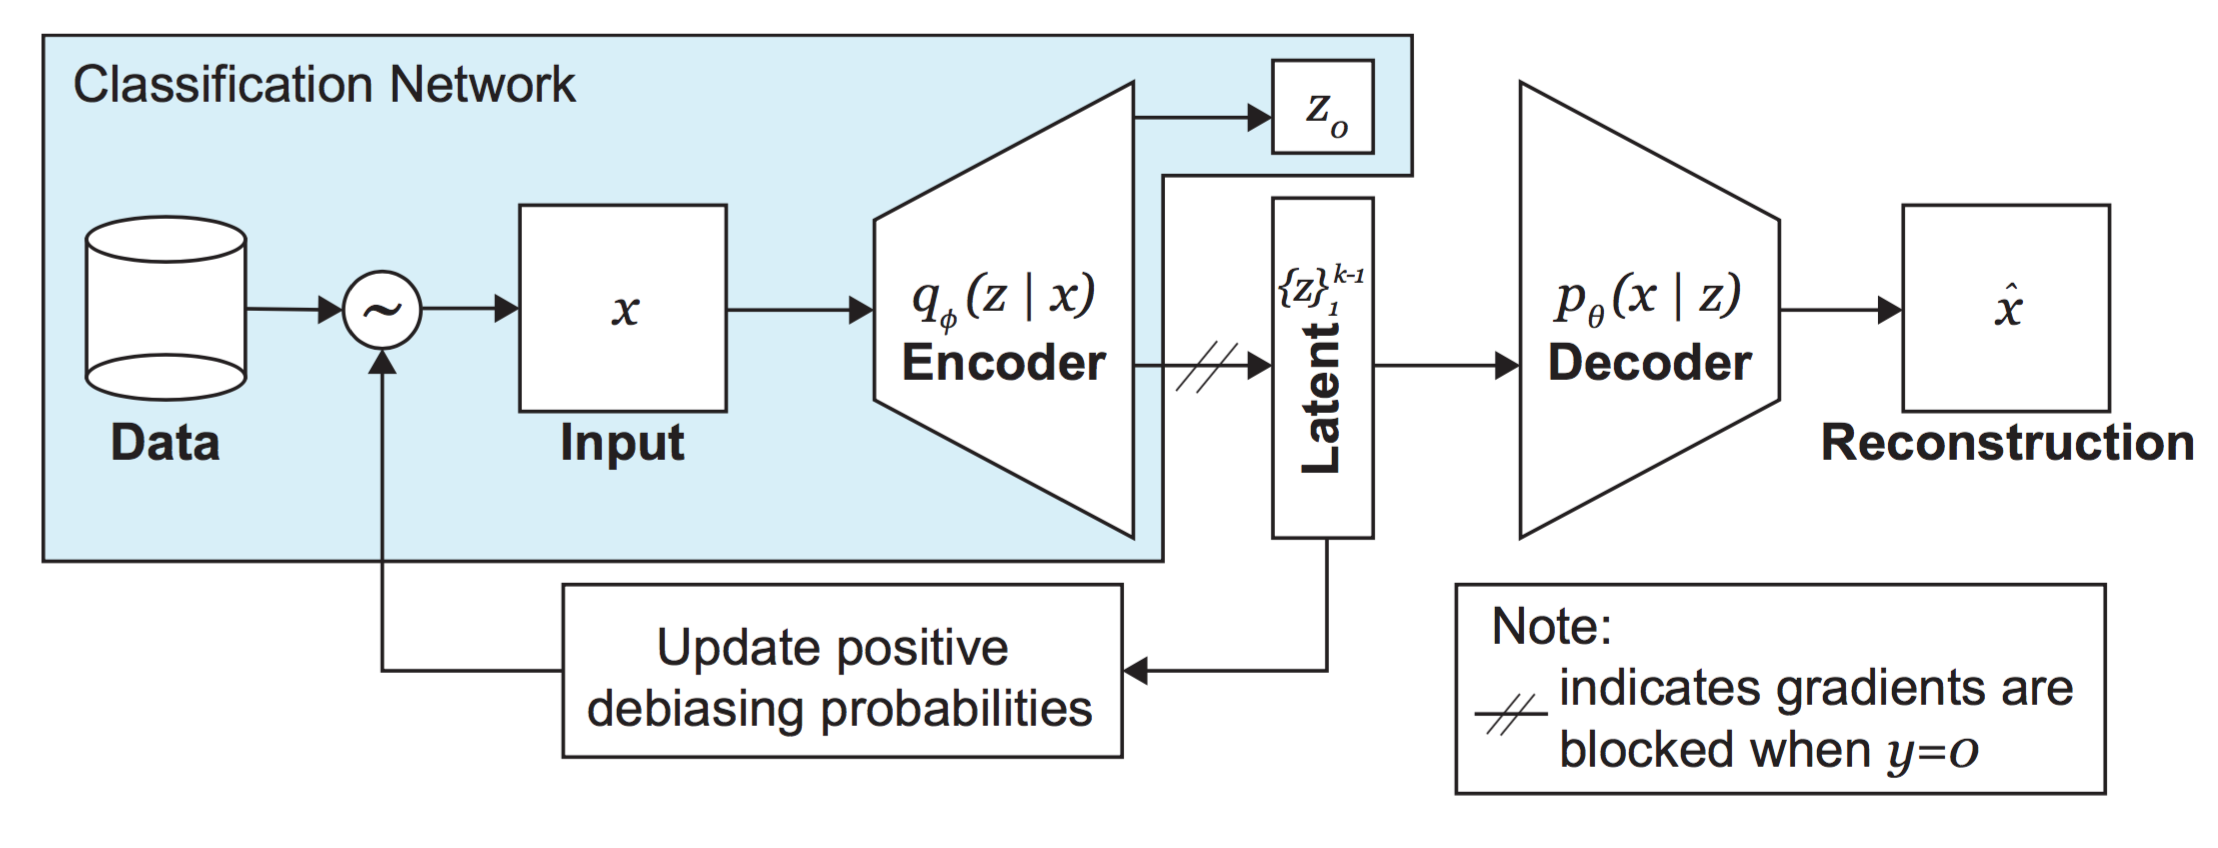
\includegraphics[width=\textwidth]{dbvae_schematic.png}
\caption{DB-VAE \cite{amini2019}. Encoder emits class variable \(z_o\) and a latent code. Gradients into the latent path are blocked when the image is not a face. Lower arrow rebuilds the probability of drawing each training face.}
\end{figure}

\subsection{Encoder and decoder}
Encoder is the standard CNN, with \(k=100\) latent variables. Its last layer emits class logit \(\hat\ell\) (the \(z_o\) of the diagram), mean, and log standard deviation. Decoder takes the sampled code through a linear layer and a series of transposed convolutions and returns a \(64\times 64\) reconstruction. Nothing in that wiring alone makes the model debiasing; that happens in the training loop.

\subsection{Faces and non-faces}
We only want a latent model of faces. Task is still binary, so non-faces have to be classified, but they should not be reconstructed through a face code. With \(I_f(y)=1\) for a face and \(0\) otherwise,
\[
L = L_y(y,\hat\ell) + I_f(y)\,L_{\mathrm{VAE}}.
\]
\(L_y\) is binary cross-entropy on the logit. At test time the decoder is ignored; deployed object is \(\hat\ell\).

Until the sampling distribution changes, this is a classifier with an auxiliary reconstruction loss. Debiasing is the arrow at the bottom of the diagram.

\section{Resampling}
\subsection{Histograms}
Once an epoch, encoder latent means are collected for every training face. For each latent variable, a histogram of ten bins estimates how faces are spread. A smoothing constant of \(0.001\) is added to bin counts. Probability of drawing a face is the inverse of the smoothed density of the bin it fell in, so under-represented regions are sampled more often and crowded regions less often. At smoothing constant \(0\), resampled training faces tend toward a uniform distribution over latent space, which is the strongest debiasing this rule gives.

\subsection{Which images are reweighted}
Each latent variable produces its own probabilities. They are combined by taking, for each face, the maximum across variables, then normalizing. Only faces are reweighted. Negative images stay uniformly sampled. Probabilities are recomputed at the start of each epoch and then held fixed for that epoch's batches.

\section{Debiased run}
\subsection{Training}
DB-VAE is trained from scratch with the same optimizer, learning rate, batch size, and two epochs as the CNN. Each epoch starts by recomputing face probabilities. Every five hundred steps the loop draws a training face next to the decoder's painting of its code. Last of those drawings:

\begin{figure}[H]
\centering
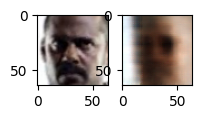
\includegraphics[width=0.38\textwidth]{dbvae_training_last.png}
\caption{Last training snapshot of the DB-VAE run. Left, a training face. Right, its reconstruction.}
\end{figure}

\subsection{Mean face probability on the test set}
\begin{figure}[H]
\centering
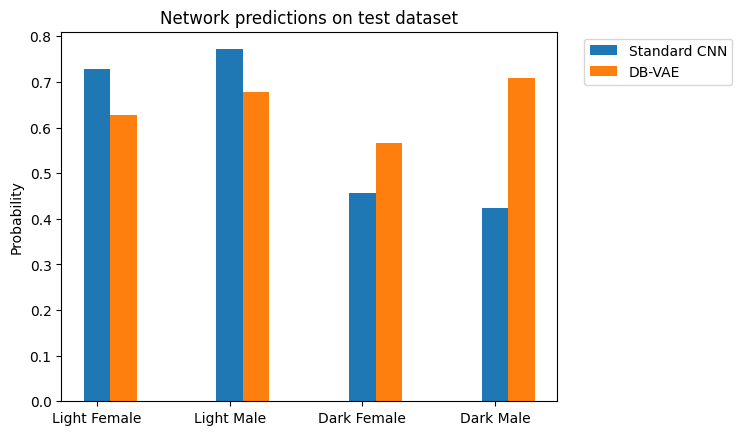
\includegraphics[width=\textwidth]{comparison_probs.png}
\caption{Mean predicted face probability by demographic group for the standard CNN and the DB-VAE.}
\label{fig:compare}
\end{figure}

Standard CNN is confident on the two light-skinned groups and much less so on the two dark-skinned groups. DB-VAE lowers mean probability on light-skinned groups and raises it on dark-skinned groups, so the four bars sit closer together.

\begin{explain}
Lower probability on light-skinned groups is part of the result. Resampling draws under-represented faces more often, so groups that dominated CelebA are seen less often than under uniform sampling.
\end{explain}

\clearpage
\section{Conclusion}
Standard CNN reaches \(99.64\%\) on a training draw and, on the demographic test set, assigns higher mean face probability to light-skinned faces than to dark-skinned faces. DB-VAE, with variational loss applied only to faces and with positives drawn from the latent resampling distribution, moves those mean probabilities toward each other across the four groups.

\clearpage
\addcontentsline{toc}{section}{References}
\begin{thebibliography}{9}
\bibitem{amini2019}
A.~Amini, A.~P.~Soleimany, W.~Schwarting, S.~N.~Bhatia, and D.~Rus.
\href{https://aies-conference.com/2019/wp-content/papers/main/AIES-19_paper_220.pdf}{Uncovering and mitigating algorithmic bias through learned latent structure}.
\emph{AIES}, 2019.

\bibitem{buolamwini2018}
J.~Buolamwini and T.~Gebru.
\href{https://proceedings.mlr.press/v81/buolamwini18a/buolamwini18a.pdf}{Gender shades: Intersectional accuracy disparities in commercial gender classification}.
\emph{FAT*}, 2018.

\bibitem{deng2009}
J.~Deng, W.~Dong, R.~Socher, L.-J.~Li, K.~Li, and L.~Fei-Fei.
\href{https://image-net.org/static_files/papers/imagenet_cvpr09.pdf}{ImageNet: A large-scale hierarchical image database}.
\emph{CVPR}, 2009.

\bibitem{liu2015}
Z.~Liu, P.~Luo, X.~Wang, and X.~Tang.
\href{https://arxiv.org/pdf/1411.7766.pdf}{Deep learning face attributes in the wild}.
\emph{ICCV}, 2015.
\end{thebibliography}

\end{document}
